%4.2.tex

\ref{chp:4_1}節で述べたLLVMのRISC-Vバックエンドでの命令生成のための命令定義クラスについて,ベクトル拡張付きRISC-Vのベクトル命令のための命令フィールドと命令の定義について述べる.

図\ref{fig:MIQSInst_class}
に定義した命令フィールド定義クラスと命令定義のためのクラスの継承関係を示す.

\begin{figure}[tb]
    \centering
    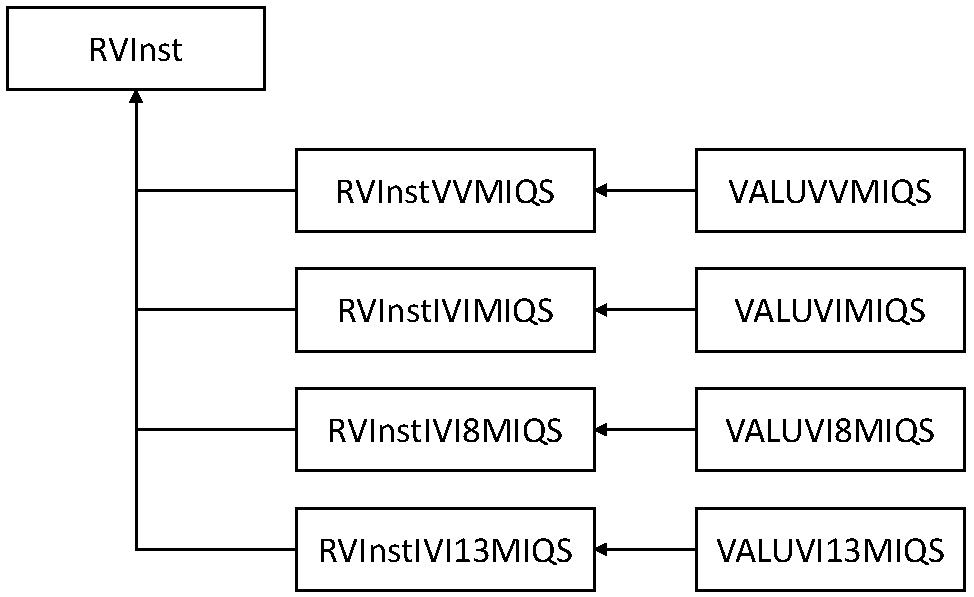
\includegraphics[scale=0.6]{image/MIQSInst_class.pdf}
    \caption{定義したクラスの継承関係}
    \label{fig:MIQSInst_class}
\end{figure}

本研究ではベクトル拡張付きRISC-Vの命令のうち,ベクトル演算命令のプレディケートレジスタを用いない命令を実装した.RISC-Vではプレディケートレジスタが用いられていないため,LLVMにもプレディケートレジスタが定義されておらず,プレディケートレジスタを用いる命令を実装するためにはプレディケートレジスタの定義に加えて,新たにレジスタ割り当て機能の実装が必要であるため,本研究ではプレディケートレジスタを用いない命令のみの実装をする.
プレディケートレジスタを用いない命令は既に実装されているRISC-VのV拡張命令のベクトル演算命令とレジスタオペランドや命令の構成がベクトル拡張付きRISC-Vのベクトル演算命令と同じ構成のため,プレディケートレジスタを用いる命令より命令生成のために必要な実装部分が少ないため,比較的容易に実装が可能である.

本研究で実装するベクトル命令とそのフォーマットを図\ref{fig:jissou_inst_format}
にまとめる.

\begin{figure}[tb]
    \centering
    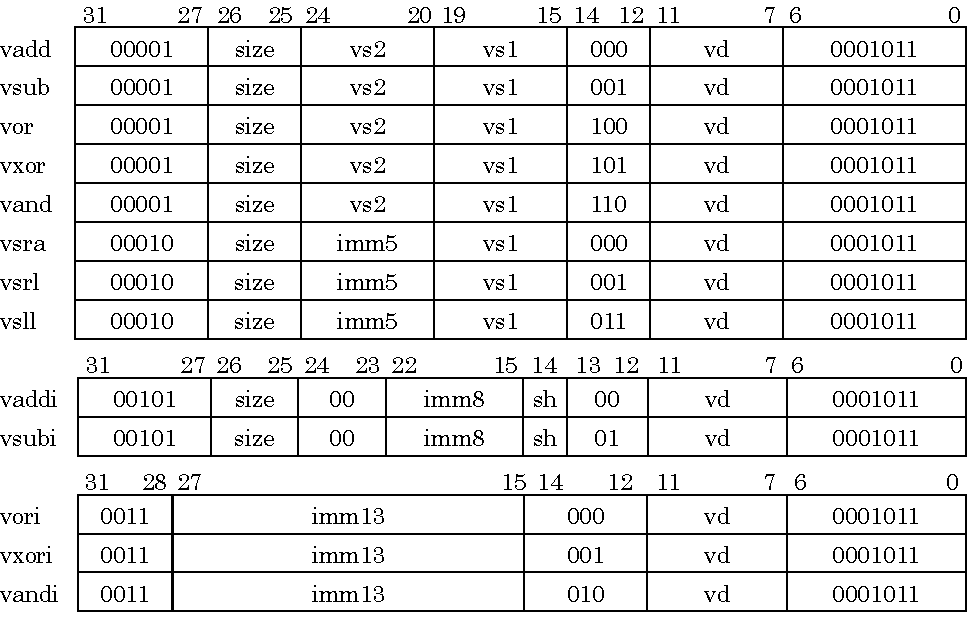
\includegraphics[scale=0.8]{image/jissou_inst_format.pdf}
    \caption{実装した命令}
    \label{fig:jissou_inst_format}
\end{figure}

図\ref{fig:jissou_inst_format}で
vaddなどの命令フォーマットのビット26および25の2ビットにて指定されているsizeはベクトル要素のサイズを指定するためのフィールドであり,この値に応じたサフィックスが命令の末尾に追加されるものである.本研究では整数要素の処理の場合のみを想定し,このsizeの値は演算を行う配列要素の大きさである32ビットサイズを表すために'0b10'で固定している.また,即値を用いた算術演算命令であるvaddi ,vsubiの命令フィールドのうちビット14のshはビット24からビット20の5ビットで指定した即値を8ビット左シフトするかを決定するためのフィールドである.このフィールドが0である場合はシフトを行わず,1であるときは8ビットのシフトを行う.このshの値はvaddi等の命令のオペランドにて指定を行うが,本研究ではシフトを行わない0で値を固定している.

実際に定義した命令フォーマットクラスの一覧を図\ref{fig:jissou_inst_format_class}
に示す.RVInstVV\_VExはvadd ,vsub ,vor ,vxor ,vandのためのベクトル算術演算命令フォーマットで.RVInstIVI\_VExは5ビットの即値を用いるvsra ,vsrl ,vsll用のベクトル論理・算術シフト演算命令フォーマット,RVInstIVI8\_VExは8ビットの即値を用いるvaddi ,vsubi用のベクトル即値間算術演算命令フォーマット,RVInstIVI13\_VExは13ビットの即値を用いるvori ,vxori ,vandi用のベクトル即値間算術演算命令フォーマットの定義である.

\begin{figure}[tb]
    \centering
    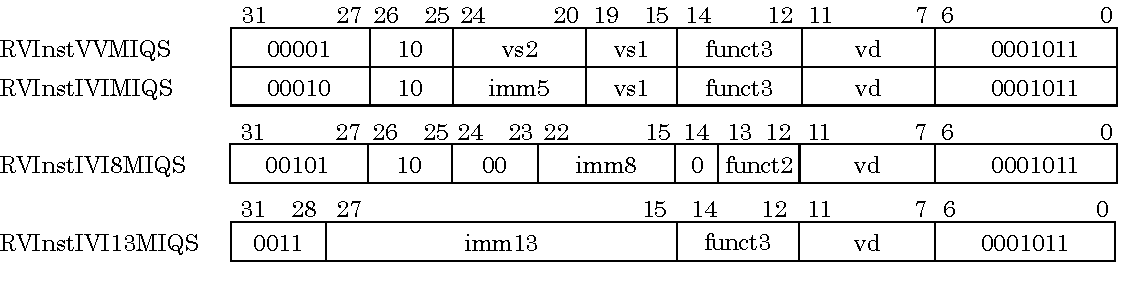
\includegraphics[scale=0.8]{image/jissou_inst_format_class.pdf}
    \caption{定義する命令フォーマットクラス}
    \label{fig:jissou_inst_format_class}
\end{figure}

また,実際のTableGenによる定義の例としてRVInstVV\_VExの定義を図\ref{fig:RVInstVVMIQS}
に示す.図\ref{fig:jissou_inst_format_class}
で示したフォーマットとなるように命令フィールドInstのどのフィールドにどの値が格納されるかを指定する.

\begin{figure}[tb]
    \centering
    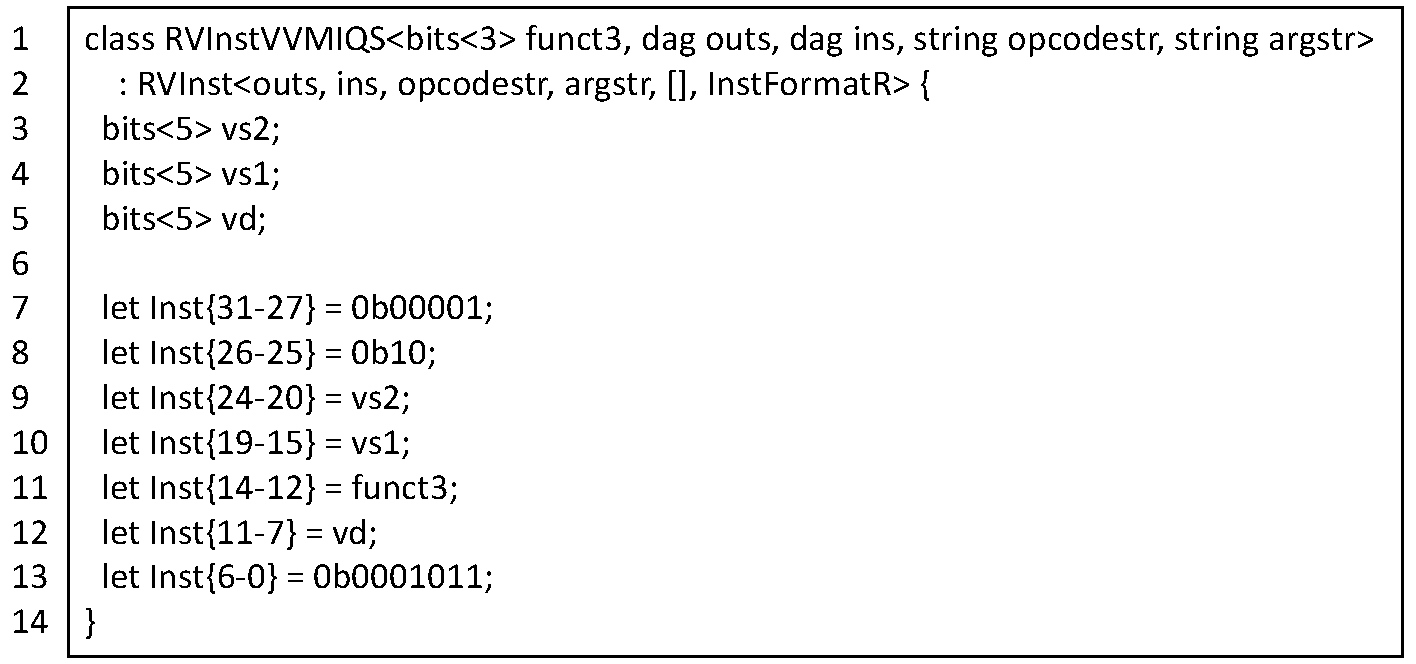
\includegraphics[scale=0.6]{image/RVInstVVMIQS_v2.pdf}
    \caption{TableGenによるRVInstVV\_VExの定義}
    \label{fig:RVInstVVMIQS}
\end{figure}

命令の定義を図\ref{fig:Inst_def}
に示す.
図\ref{fig:Inst_def}
のALUVV\_VExはベクトル同士の演算を行うための命令の定義用に定義の繰り返しを行わないためのクラスである.ALUVV\_VExでは出力レジスタと入力レジスタの指定を行う.このクラスを定義することで例えば\textit{vadd.w vd vs1 vs2}と\textit{vsub.w vd vs1 vs2}のようにオペランドが同じ命令の定義を行う場合,ALUVV\_VExをインスタンス化する際に入出力レジスタの定義を繰り返しを防ぐことができる.

命令のインスタンス化も図\ref{fig:Inst_def}
で行っている.ベクトル算術・論理演算命令のインスタンス化を行っている.引数では命令の文字列と命令選択のための値を指定している.

\begin{figure}[tb]
    \centering
    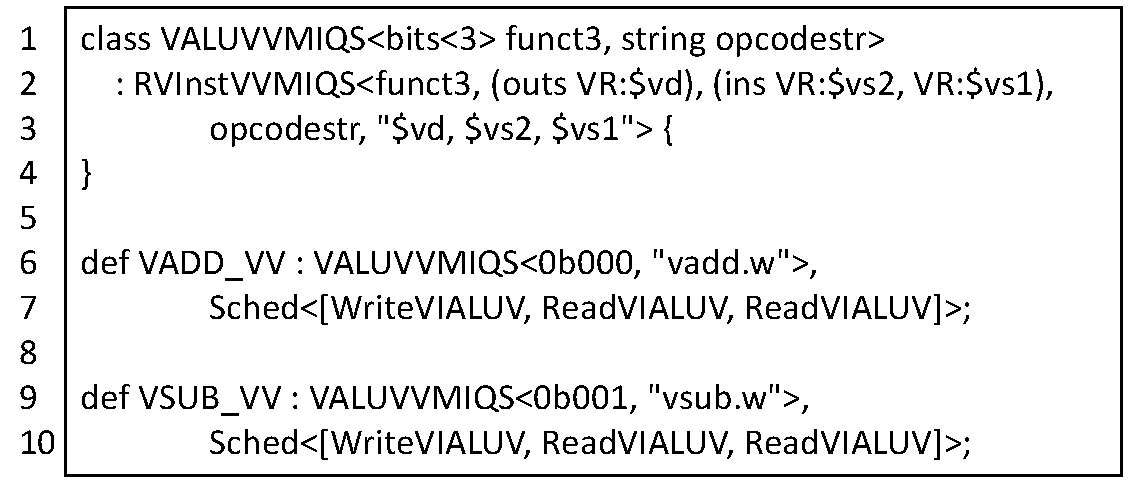
\includegraphics[scale=0.6]{image/Instruction_define.pdf}
    \caption{命令の定義}
    \label{fig:Inst_def}
\end{figure}

TableGenによる命令の定義は以上のように行われ,残りの命令フォーマットや命令についても同様に定義を行う.
